% Nikolai Nielsens "Fysiske Fag" preamble
\documentclass[a4paper,10pt]{article} 	% A4 papir, 10pt størrelse
\usepackage[english]{babel}
\usepackage{Nikolai} 					% Min hjemmelavede pakke
\usepackage[dvipsnames]{xcolor}

% Margen
\usepackage[margin=1in]{geometry}

% Max antal kolonner i en matrix. Default er 10
%\setcounter{MaxMatrixCols}{20}

% Hvor dybt skal kapitler labeles?
%\setcounter{secnumdepth}{4}	
%\setcounter{tocdepth}{4}


% Hvilket nummer skal der startes med i sections? (n-1)
%\setcounter{section}{0}	

% Til nummerering af ligninger. Så der står (afsnit.ligning) og ikke bare (ligning)
\numberwithin{equation}{section}


% Header
%\usepackage{fancyhdr}
%\head{}
%\pagestyle{fancy}

%Titel
\title{Numerical Methods in Physics Week 2}
\author{Nikolai Plambech Nielsen}
\date{}

\begin{document}
	\maketitle
	\section{Diffusion}
	For this assignment, diffusion from an initial delta-function peak is evaluated numerically. The differential equation is the diffusion equation, which in one dimension is
	\begin{equation}\label{key}
		\diff{C}{t} = D \diff{^2 C}{t^2}
	\end{equation}
	where $ D $ is the diffusion constant. This is a partial differential equation which necessitates the use of other methods. For evaluating the time derivative, simple Euler integration can be used, but for evaluating the double space derivative, a new method is used. First, space needs to be discretized, which allows one to calculate the derivative similarly to Euler integration. The integration scheme is called Forward in Time Centered in Space (FTCS), which for this equation uses 3 points at the last time step, to compute the value at each point in the next time step. To evaluate the $ j $'th point in space, the $ j-1 $'th, $ j $'th and $ j+1 $'th point, all from the last time step, is used. Numerically this is
	\begin{equation}
		C^{n+1}_j = C^n_j + \frac{D \Delta t}{h^2} (C^n_{j-1}+C^n_{j+1} - 2 C^n_j),
	\end{equation}
	where $ h $ is the distance between each point in space, equivalent to $ \Delta t $ in time.
	
	To numerically evaluate the delta-function, the following numerical equivalent is used
	\begin{equation}\label{key}
		\delta(x-x_0) \to \begin{cases}
		1/h & x = x_0 \\
		0 & x \neq 0,
 		\end{cases}
	\end{equation}
	as this is a sharp peak around $ x_0 $ and "integrating" this over all space gives 1:
	\begin{equation}\label{key}
		\sum \delta(x-x_0) h = \sum_{x_0}^{x_0} \frac{h}{h} = 1
	\end{equation}
	For simplicity, $ x_0 = 0 $ is used for all the following assignments. The analytical solution to this problem is
	\begin{equation}\label{key}
		C(x,t) = \frac{1}{\sigma(t) \sqrt{2\pi}} \exp\pp{-\frac{(x-x_0)^2}{2\sigma(t)}}, \quad \sigma(t) = \sqrt{2Dt}.
	\end{equation}
	which is a delta function in the limit of $ t\to 0 $, but spreads out as time passes.
	
	However, the choice of $ N $ might pose a small problem, if the $ x $-interval is centred around $ x=0 $. If there is an odd number of points, the middle-most point will definitely be $ x=0 $, but if there is an even number of points, this is not the case. $ x= 0 $ will lie directly between two points. To prevent any discrepancy, the delta-function is modified for even values of $ N $:
	\begin{equation}\label{key}
	\delta(x-x_0) \to \begin{cases}
	1/2h & x=x_0\pm h/2 \\
	0 & \text{otherwise}
	\end{cases}, \ (\text{for equal } N).
	\end{equation}
	
	To compare the numerical and analytical solutions, the following values are used: $D = 0.1, L = 2\pi,N=128 $, with $ h=L/(N-1) $ as this is the spacing MATLAB uses with the \texttt{linspace} function, and $ \Delta t = h^2/4D $. The positions after $ t = 1 $ are plotted, along with the difference between the two solutions
	\begin{figure}[H]
		\centering
		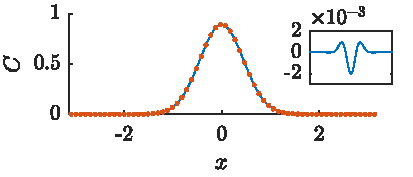
\includegraphics[width = 0.5\linewidth]{diffSimple.pdf}
		\caption{The numerical (blue line) and analytical (orange points) solutions to the diffusion equation for a delta function initial condition. An inset of the difference between the numerical and analytical solutions is also shown.}
		\label{fig:diffSimple}
	\end{figure}
	The analytical and numerical solution to the differential equation are in agreement, with a max difference of $ 2.04\D10^{-3} $. However, at the edges of the simulation, where both solutions are approximately zero, the fractional error does exceed 0.5 at places.
	
	Next the relation between error, grid size and time step size is explored. However, comparing errors between simulations with different grid sizes becomes difficult, as this does not allow for easy plotting. Therefore the error on the final time step is summed up and divided by the number of points to normalize the error. First the simulation is run with 128 points, for 1 unit of time, with 100 linearly spaced values of $ \Delta t $ between $ h^2/2D $ and $ h^2/100D $. Next the simulation is run with between 20 and 1000 points in increments of 20, with $ \Delta t = h^2/4D $, where $ h = L/(N-1) $, to satisfy the stability condition. The results are shown in the figures below:
	 
	\begin{figure}[H]
		\centering
		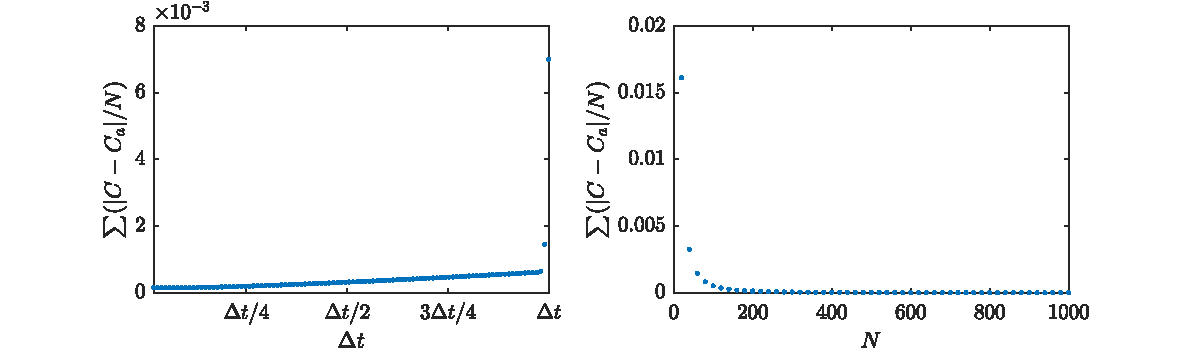
\includegraphics[width = \linewidth]{diffErr.pdf}
		\caption{Plots of the normalized cumulative error as a function of the time step size $ \Delta t $ (left) and grid size $ N $ (right). On the right plot, the grid size is $ N = 128 $, and on the left plot, the time step is $ \Delta t = h^2/4D $.}
		\label{fig:diffErr}
	\end{figure}
	
	
\end{document}

